\documentclass[12pt]{article}
\usepackage{hyperref} % lien tableofcontents + url
\usepackage{graphicx} % pour les images
\usepackage{float} % pour le [H] des figures
\usepackage[utf8]{inputenc}
\usepackage[T1]{fontenc}
\usepackage{listings}
\usepackage{hyperref}

\usepackage{subcaption}

\usepackage{csvsimple}

\topmargin -1.1in 
\textheight 9.7in
\setlength{\textwidth}{7.5in}
\oddsidemargin = -.5in

\begin{document}

\title{Rapport technique \\ Application Vélo Épicurien}
\author{MANZAMBI Sean \\ SESBOÜÉ Matthias \\ SASSEVILLE Martin}

\maketitle

\begin{abstract}
    Le présent rapport décrit la réalisation de l'application Vélo épicurien. Cette application permet à un usager, amateur de vélo et de bonne bouffe, d'obtenir un parcours via les pistes cyclables, qui lui permettent d'effectuer un certain nombre d'arrêts dans des restaurants proposant ses types de cuisine préférés.
\end{abstract}

\section{Présentation des données utilisées pour le projet}

\subsection{Source et taille des données}

    Afin de supporter l'application, il est essentiel de disposer de données sources exploitables qui permettront d'obtenir un parcours cyclable ainsi que des restaurants à proximité de ces pistes cyclables. 
    
    Dans un premier temps, les données pour les pistes cyclables seront obtenues via \href{https://www.donneesquebec.ca/recherche/fr/dataset/vque_24}{les données publiques de la ville de Québec}. Cette base de données contient $30 949$ points géographiques délimitant l'ensemble des plus de de $485$ kilomètres de pistes cyclables sur le territoire de la ville de Québec. Pour les données relatives aux restaurants, elles seront obtenues par une méthode d'extraction de données (web scrapping) à partir du \href{https://www.restoquebec.ca/}{site web de Resto Québec}. La base de données créée contient $2 496$ restaurants répartis tout autour de la ville de Québec.

    Les données sont extraites au format GeoJSON afin de faciliter leur intégration dans les bases de données, qui gèrent nativement ce format (voir \href{https://geojson.org/}{le site geojson.org} pour les détails de ce format).

\subsection{Analyse descriptive des données}

    Ces bases de données ont été choisies car elles contiennent les informations essentielles au bon fonctionnement de l'application. En effet, celle-ci doit pouvoir retourner une série de lieux (nom du lieu et/ou ses coordonnées) ordonnancés afin de décrire un trajet d'une longueur maximale spécifiée, ainsi que les restaurants (nom du restaurant et/ou ses coordonnées) situés  sur ce parcours pour le nombre d'arrêts souhaités. 
    
    Les bases de données supportant cette application doivent donc contenir à minima les informations suivantes :

    \begin{itemize}
        \item Pour les pistes cyclables
        \begin{itemize}
            \item le nom du lieu
            \item les coordonnées géographiques de ce lieu
        \end{itemize}
        \item Pour les restaurants
        \begin{itemize}
            \item nom
            \item adresse
            \item coordonnées géographiques
            \item type(s) de cuisine
        \end{itemize}
    \end{itemize}

    Les données GeoJSON extraites contiennent, en plus des types de géométries et des coordonnées des points, les informations suivantes :
     \begin{itemize}
         \item Pour les pistes cyclables
         \begin{itemize}
             \item nom de la topographie (nom de rue, avenue, boulevard ...)
             \item type de voie
             \item si cette voie est à sens unique ou non
             \item la longueur de la voie
         \end{itemize}
         \item Pour les restaurants
         \begin{itemize}
             \item nom du restaurant
             \item adresse
             \item prix moyen du restaurant sous forme d'une échelle allant de 1 à 4 symboles \$
             \item les types de nourritures servis dans le restaurant
         \end{itemize}
     \end{itemize}

\section{Technologies utilisées pour le projet}

\subsection{Langage de programmation et bibliothèques}

    Le langage de programmation qui a été choisi pour l'application est le Python, dans sa version 3.6. C'est un langage très utilisé qui propose un grand nombre de bibliothèques matures, qui seront utiles pour implémenter les différentes interfaces nécessaires.

    Les bibliothèques suivantes sont utilisées :

    \begin{itemize}
        \item Flask est un framework open-source de développement web en Python. Son but principal est d'être léger, afin de garder la souplesse de la programmation Python, associé à un système de templates. Il permet de développer rapidemment et facilement une API web pour interfacer avec les bases de données.
        \item Pymongo est l'API python qui met à disposition tous les outils nécessaires pour faire des requêtes sur une base de données MongoDB.
        \item Py2neo est l'API python qui met à disposition tous les outils nécessaires pour faire des requêtes sur une base de données Neo4J.
        \item json est un module python permettant de manipuler les fichiers au format JSON. 
    \end{itemize}

\subsection{Bases de données}

    La base de données MongoDB orientée document est utilisée pour stocker les informations concernant les restaurants. Les données géographiques, des restaurants ainsi que celles des pistes cyclables, seront stockées dans la base de données orientée graphe, Neo4J.

\subsection{Modélisation des données en BD}

\subsubsection{Base de données MongoDB}

    Les données concernant les restaurants sont importées telles quelles dans la base de données MongoDB. Notons que seules les données relatives au restaurant lui même et non relatives à sa position sont importées. La base de données MongoDB ne contient que ces données.

\subsubsection{Base de données Neo4J}

    Les données géographiques demandent une étape de pré traitement. Dans un premier temps les points des pistes cyclables sont extraits. Dans le fichier GeoJSON, ces derniers sont intégrés à des formes géographiques de type "LineString" qui se recoupent parfois. L'extraction de ces points permet d'éliminer les doublons, d'intégrer ces points dans les sommets du graphe de la base de données orientée graphe, en plus de faire des calculs à partir de ces points.

    Ces points permettent ensuite de calculer, d'une part les intersections entre les lignes brisées que forment les suites de points, et ainsi d'introduire de nouveaux points essentiels. D'autre part ils permettent de calculer, à partir de l'ensemble des points, quel restaurant est plus proche de quel point (dans une limite de 500 mètres d'un point). Ainsi, chaque restaurant est assigné à un seul point.
    
    Pour résumer, la base de données Neo4J contient comme présenté dans la figure \emph{figure~\ref{actual_neo_model} page~\pageref{actual_neo_model}} :

    \begin{itemize}
        \item Un ensemble de sommets représentant les points des pistes cyclables. Ces sommets ont pour propriétés une longitude, une latitude ainsi qu'un identifiant unique et le nom de la topographie à laquelle le point appartient (nom de la rue, avenue, piste cyclable \dots)
        \item Les sommets de cet ensemble sont reliés par des arrêtes bidirectionnelles s'il existe une route entre les points. Ces arrêtes ont un attribut "distance" contenant la distance entre les deux points
        \item Un ensemble de sommets représentant les points des restaurants. Ces sommets ont pour attributs, le nom et l'adresse du restaurant qui servent à reconnaître le restaurant de façon unique
        \item Ces sommets "restaurant" sont reliés à leur point de piste cyclable le plus proche.
    \end{itemize}
        
    \begin{figure}[h]
        \centering
        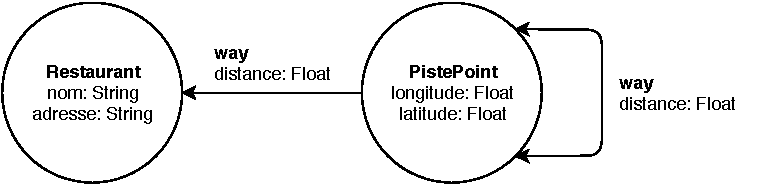
\includegraphics[scale=1]{images/actual_neo_model.pdf}
        \caption{\label{actual_neo_model} Visualisation du modèle de données de la BD Neo4J}
    \end{figure}

\section{Algorithme permettant de produire les parcours}

\subsection{Communication des valeurs calculées entre les bases de données}

    Lorsque l'utilisateur sélectionne la liste des types de restaurants où il souhaite manger sur son parcours, l'ensemble des noms de restaurants servant de la nourriture d'un type de cette liste est extrait depuis la base de données MongoDB contenant les informations sur les restaurants. Cet ensemble de restaurants est utilisé ensuite en paramètre dans la requête faite à la base de données Neo4J pour extraire le meilleur chemin.
    Une fois la liste des restaurants choisis il est facile d'extraire de la MongoDB les informations complémentaires souhaitées.

\subsection{Calcul permettant de trouver le parcours épicurien le plus intéressant pour l'usager}

    Dans un premier temps, un point de départ est extrait de manière aléatoire à partir de chemins calculés correspondants aux contraintes de distance maximale à parcourir et du type de nourriture que l'utilisateur souhaite manger.
    Ce point de départ est ensuite utilisé pour calculer un parcours qui part d'un point situé dans un rayon de 500 mètres autour du point de départ. Pour finir, l'extraction de la liste de points formant le parcours est laissée au programme de la base de données Neo4J. Littéralement, nous demandons à Neo4J, via une requête Cypher, "extrait une liste de points reliés deux à deux, dont le premier point est le point de départ, certains de ces points sont reliés à des restaurants de l'ensemble spécifié et la somme des distances entre ces points est inférieure à la distance maximale".  

\section{Documentationd de l'API}

    L'API propose actuellement les requêtes suivantes via des méthodes GET:

    Page d'acceuil :

    \begin{lstlisting}
        @GET /

        returns: "Bonjour et bienvenu dans notre application de velo epicurien"
    \end{lstlisting}

    Statistiques de bases sur les bases de données :

    \begin{lstlisting}
        @GET /heartbeat

        returns:
        {
            "nb_restaurants":int,
            "total_path_length":float
        }
    \end{lstlisting}

    Le README correspondant à cette documentation :

    \begin{lstlisting}
        @GET /readme
        
        returns: Cette documentation en markdown
    \end{lstlisting}

    Liste des types de restaurant existants :
    
    \begin{lstlisting}
        @GET /type

        returns:
        [
            str,
            str,
            str,
            ...
        ]
    \end{lstlisting}

    Obtenir un point de départ : 

    Dans le navigateur, on met les paramètres dans l'URL, maximum\_lenght='distance' et type='liste de types de restaurant'. Les types sont séparés par le signe '+', exemple http://localhost:8080/starting-point?maximum\_length=100\&type=Sandwichs+Casse-croute

    \begin{lstlisting}
        @GET /starting-point
        {
            "maximum\_length": int (en metre),
            "type": [str, str, ... ]
        }

        returns:
        {
            "starting\_point" : {
                                    "type":"Point", 
                                        "coordinates":{
                                            "latitude":float, 
                                            "longitude":float
                                    }
                                }
        }
    \end{lstlisting}


    Générer un parcours :
    
    Dans le navigateur, on sépare les types pas des symboles '+' dans l'url, exemple http://localhost:8080/parcours?maximum\_length=500\&type=Sandwichs+Poutine\&number\_of\_stops=1
        
    \begin{lstlisting}
        @GET /parcours
        {
            "starting\_point" : {
                                    "type":"Point", 
                                    "coordinates":{
                                        "latitude":float, 
                                        "longitude":float
                                    }
                                },
            "maximum\_length": int (en metre),
            "number\_of_stops": int,
            "type": [str, str, ... ]
        }

        returns:
        [
            {
                "segment\_id":1,
                path: {
                    type:"LineString", 
                    "coordinates":{
                        "latitude":float, 
                        "longitude":float
                    }
                },
                restaurant: {
                    "name": string,
                    "type": string,
                    "cote": float,
            },
            {
                "segment\_id":2,
                ....   
            }
        ]
    \end{lstlisting}
    
\section{Plan d'expansion}

\subsection{Point de départ}

    Le MVP présenté ici est une preuve de concept. Il peut être amélioré de beaucoup de manières différentes.

    Il est a noter que actuellement seulement une partie des données à disposition est utilisée. En effet, pour l'instant, les informations comme le type de voie, le sens unique ou non d'une voie, l'ordre de prix d'un restaurant \dots ne sont pas utilisées.

    L'API présentée ici se veut simple et ne fournit que les fonctionnalités minimales. Dans le futur, plus de fonctionnalités seront ajoutées.

\subsection{Gestion de l'évolution des volumes de données (Scalabilité)}

    Avant d'apporter de nouvelles fonctionnalités, il faut s'assurer que l'application sera capable de répondre aux requêtes d'un nombre croissant d'utilisateurs. Pour cela, plusieurs évolutions à mettre en place ont été identifiées, que ce soit au niveau de la modélisation des données comme au niveau de l'architecture logicielle.

    La modélisation des données peut être améliorée de deux manières :

    \begin{figure}[h]
        \centering
        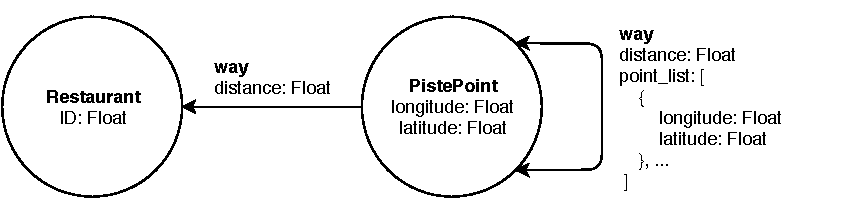
\includegraphics[scale=1]{images/updated_neo_model.pdf}
        \caption{\label{updated_neo_model} Modèle de données optimisé pour la BD Neo4J}
    \end{figure}
    
    \begin{itemize}
        \item Un identifiant unique doit être créé pour chaque restaurant et partagé entre la base de données MongoDB et celle Neo4J. Ce dernier permettra de réellement stocker toutes les informations relatives aux restaurants, autres que les coordonnées, dans la MongoDB. Et ainsi éviter de dupliquer des données et alléger la quantité de données dans la Neo4J.
        \item Toujours dans un objectif d'optimisation des données stockées dans la Neo4J, une réorganisation des points peut être faite. En effet, actuellement chaque point est stocké comme un sommet mais cela n'est pas utile pour tous. Les points ne servant que d'intermédiaires entre deux points ne nécessitent pas de créer un sommet, et leurs coordonnées peuvent simplement être stockées sous forme d'une liste dans un attribut de l'arrête liant les deux extrémités d'une ligne comme présenté dans la figure \emph{figure~\ref{updated_neo_model} page~\pageref{updated_neo_model}}. Cela est donc valable pour tous les points qui ne sont ni reliés à un restaurant, ni une intersection, c'est à dire reliés à plus de deux autres points.
    \end{itemize}

    D'un point de vue architectural les possibilités suivantes sont considérées :

    \begin{itemize}
        \item L'application est tout d'abord lancée en phase de test sur la ville de Québec. Un seul centre de données est actuellement nécessaire, positionné le plus proche possible de la ville de Québec étant donné que la majorité des utilisateurs seront dans cette zone.
        \item En termes de réplication, une approche "single-leader" avec réplication asynchrone est considérée. En effet la majorité des requêtes seront des lectures. Celles en écritures seront principalement l'ajout de nouveaux points pour les pistes cyclables ou les restaurants Si un utilisateur ne reçoit pas immédiatement un chemin incluant ces changements, cela n'est pas critique.
        \item En fonction du développement spatial de l'application, une approche "multileader" toujours avec réplication asynchrone pourra être considérée à mesure de la création de nouveaux centres de données. Ces centres seront placés en fonction des zones (par exemple, Amérique centrale, Amérique du nord \dots) pour répartir les flux de données. Cette répartition par zone permettra également d'optimiser la réplication des données par zone. C'est à dire de répliquer en priorité les modifications faites sur une zone dans son cluster correspondant.
        \item Lors de l'expansion, la position de ces centres de données devient importante au niveau de la gestion des données personnelles. En effet, actuellement chaque pays impose des contraintes différentes sur la gestion de ces données. Le fait d'avoir à minima un centre différent par pays permet d'appliquer ses contraintes de manière plus précise. 
        \item Cette architecture sera à adapter lorsqu'une gestion de profils utilisateurs, fil d'actualité, ou encore d'évaluation des restaurants ou des parcours, sera mise en place.
        \item Lorsque la quantité de données à gérer atteindra un volume trop important une approche de partionnement par hash de clés sera considéré. Les requêtes ne portent pas sur des plages de données mais plutôt sur des données précises.
        \item Avec l'ajout de nouvelles fonctionnalités comme la gestion des utilisateurs ou la proposition des chemins personalisés, une approche de partionnement sur les indexs secondaires par terme sera alors considérée. Cela permettra de répondre de manière optimisée à des requêtes comme "trouve tous les restaurants que cet utilisateur a déjà visité". Encore une fois les écritures sont moins fréquentes que les lectures, il est donc plus intéressant d'optimiser le partionnement sur les lectures. 
    \end{itemize}

\subsection{Fonctionnalités additionnelles envisagées}

    \subsubsection{Fonctionnalités de base}

        Dans un premier temps il est primordial d'ajouter une gestion de profils utilisateurs ainsi qu'un système de géolocalisation. Cela permettra d'offrir un service de bien meilleure qualité, plus personalisé, et produira des données essentielles pour l'utilisation de méthodes d'analyses de données nécessaires à cette personnalisation du service.

        Une fois les profils d'utilisateurs créés, un système de notation des restaurants et une liste des restaurants déjà visités seront ajoutés. De plus, les trajets déjà effectués seront conservés pour chaque utilisateur.

    \subsubsection{Fonctionnalités à plus long terme}

        À plus long terme, un sytème de recommandations équivalent à celui de Netflix pour ces films, sera implémenté pour proposer par défaut des trajets aux utilisateurs en fonction de leurs trajets précédents et des types de nourriture qu'ils préfèrent. Ces recommandations se baseront dans un premier temps, sur la longueur maximale des trajets précédemment effectués par l'utilisateur, mais aussi sur ses types de nourriture préférés et de la polarité des commentaires laissés sur les restaurants. 

        L'idée principale est de faire évoluer l'application d'un simple outil à un réseau social. Une fois les fonctionnalités précédentes implémentées et stables, un fil d'actualité sera ajouté, et les utilisateurs pourront ajouter des amis. Cela permettra d'une part aux restaurateurs de proposer des rabais ou des évènements spéciaux, et d'autre part, aux utilisateurs de partager leurs trajets et leurs commentaires sur ceux-ci. Ces informations seront ajoutées au fil d'actualité.

        Enfin, des méthodes de gamification seront utilisées et un tableau des scores sera ajouté présentant une balance entre les calories consommées par la pratique du vélo et celles emmagasinées par la consommation de nourriture.

\end{document}
